\chapter{Przegląd obecnych rozwiązań}
\label{chapter-2}

W rozdziale zaprezentowano konstrukcje podobne do realizowanego urządzenia oraz przedstawiono jego ogólną zasadę działania.

\vspace{0.5cm}

\section{Rozwiązania dostępne na rynku komercyjnym}

%Wykonując pomiary przetwornic napięciowych najczęściej korzysta się ze standardowego zasilacza laboratoryjnego oraz obciążenia aktywnego.
%Urządzenia te wymagają jednak często ręcznej zmiany ich ustawień i ręcznego zapisu danych pomiarowych. W celu przyspieszenia tego procesu,
%wielu producentów sprzętu laboratoryjnego umożliwia podłączenie swoich urządzeń do komputera poprzez dedykowany interfejs (LAN, RS232, USB), a następnie
%kontrolę przy pomocy dedykowanej aplikacji, czy też programowanie, np. wykorzysując środowisko LabView. Daje to możliwość stworzenia dedykowanej aplikacji,
%która to mogłaby realizować automatyczne pomiary przetwornic. Wymaga to jednak sporo czasu poświęconego na odpowiednie ustawienie sprzętu, programowanie, a także
%niekiedy wymaga zakupu sprzętu od konkretnego producenta. Należy bowiem zaznaczyć, że nie wszystkie urządzenia tego typu umożliwiają pomiar 
%wszelkich potrzebnych nam parametrów.

Obecnie na rynku możemy znaleźć urządzenia, które integrują w sobie komponenty niezbędne do realizacji omawianego problemu pomiaru parametrów przetwornic.
Za przykład służyć może m.in. N6705C od firmy Keysight \cite{n6705c}, przedstawiony na zdjęciu \ref{fig:N6705C}.

\begin{figure}[h!]
    \centering
 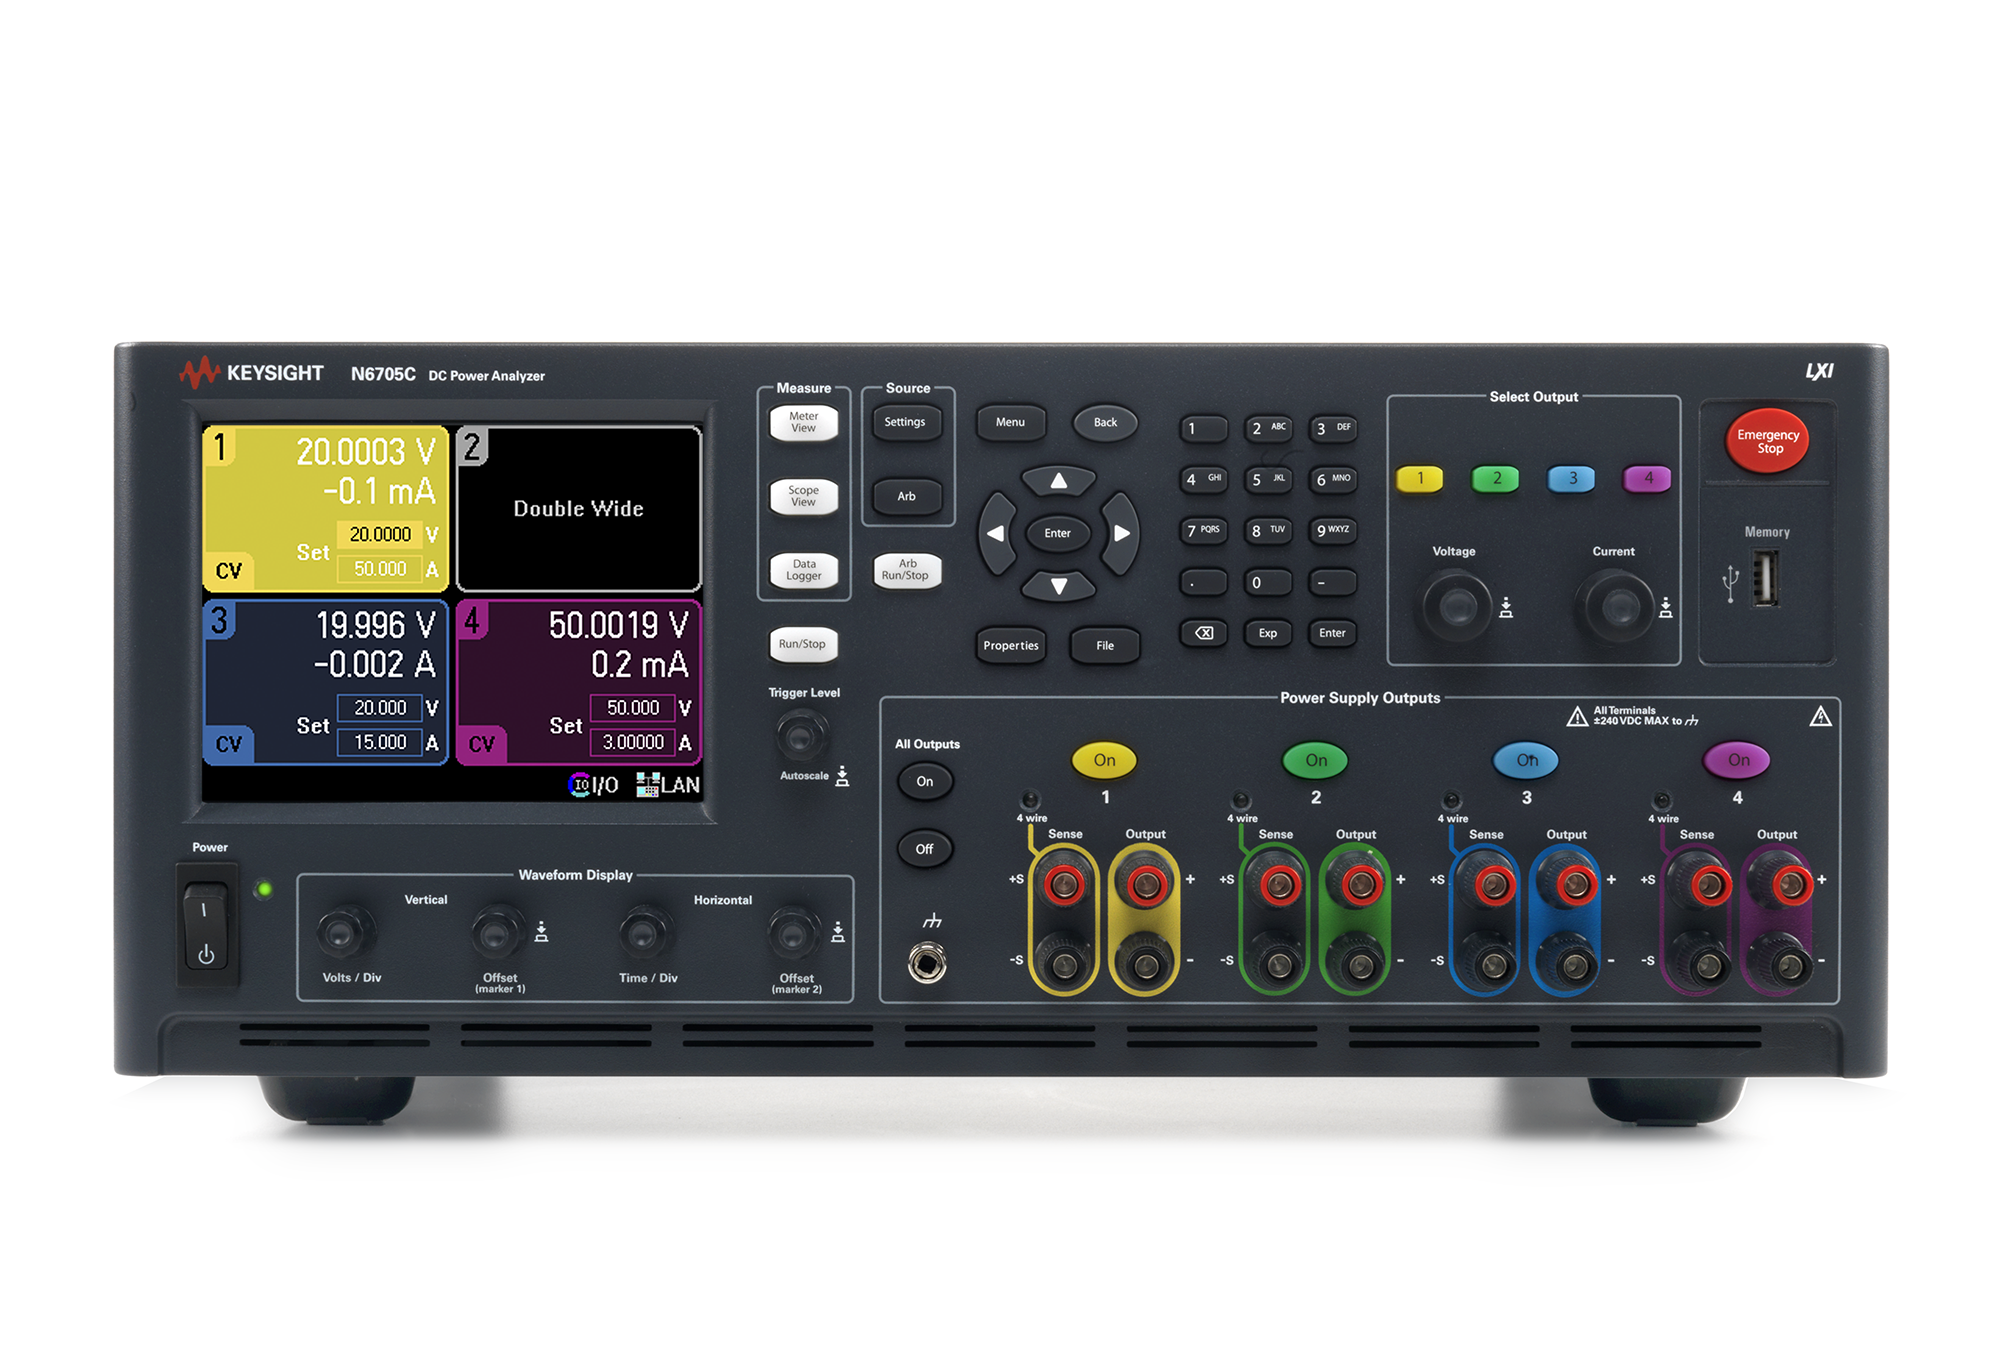
\includegraphics[width = 15cm]{images/n6705c.png}
 \caption{N67005C firmy Keysight.}
 \label{fig:N6705C}
\end{figure}

Przedstawione urządzenie posiada funkcje oscyloskopu, precyzyjnego woltomierza, miernika prądu, generatora funkcyjnego oraz logowania danych.

Kolejną opcję stanowią tzw. Bidirectional Power Supplies, jak np. te od firmy ElektroAutmatik \cite{bidirectional_DC_PSU}. 
Poniżej \ref{fig:ElektroAutomatik} widoczne jest jedno z takich urządzeń.


\begin{figure}[h!]
    \centering
 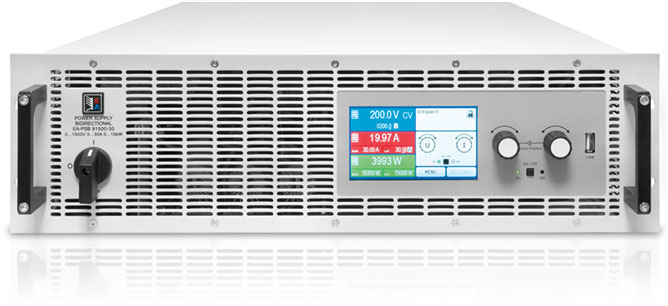
\includegraphics[width = 15cm]{images/elektroautomatik.jpg}
 \caption{Przykładowy zasilacz dwukierunkowy od ElektroAutmatik.}
 \label{fig:ElektroAutomatik}
\end{figure}

Takie przyrządy integrują w sobie zasilacze DC - najczęściej przetwornice impulsowe o dużej mocy - oraz obciążenie aktywne.
Pozwala to na pomiar mocy wyjściowej i wejściowej. Znaleźć można urządzenia tego typu od różnych producentów, różniące się parametrami, obudową (w tym przypadku typu rack), czy też interfejsami komunikacyjnymi.

Cechą wspólną obu zaprezentowanych rozwiązań jest niestety ich wysoka cena. Są to narzędzia dla specjalistów, mające wąski zakres zastosowań, w związku z czym ciężko jest znaleźć podobne instrumenty w budżecie kilku lub kilkunastu tysięcy złotych.
Kolejną wadą może okazać się brak możliwości modyfikacji, zarówno sprzętu, jak i oprogramowania. Użytkownik nie ma pełnej kontroli nad działaniem swojego sprzętu, co w niektórych wypadkach utrudnia przeprowadzenie wymaganych testów, bądź pomiarów.



%Na rynku powstały już zintegrowane urządzenia, zawierające w sobie niezbędne komponenty, takie jak zasilacz regulowany i obciążenie aktywne.
%Przykładem jest tu N6705C od firmy Keysight [TODO: DODAĆ ZDJĘCIA + REFERENCJA DO ŹRÓDŁA (https://www.keysight.com/us/en/product/N6705C/dc-power-analyzer-modular-600-w-4-slots.html)]
%Urządzenie to pozwala na wykonywanie pomiaru sprawności przetwornic napięciowych i przesłanie danych do komputera w celu dalszej ich analizy.
%Wadą takiego rozwiązania jest jednak cena przedstawionego urządzenia, a także zamknięte oprogramowanie, które nie pozwala na wprowadzanie własnych modyfikacji.
%Zamyka to możliwość na samodzielne rozszerzanie funkcjonalności takiego produktu.
%...

\section{Alternatywne rozwiązania}

Chcąc pozbyć się problemu ceny oraz braku możliwości dostosowywania urządzeń do wymagań użytkownika, inżynier może zdecydować się na zbudowanie własnego stanowiska testowego, służącego pomiarowi parametrów przetwornic napięciowych.
Jak już wspomniano, w tym celu można wykorzystać zasilacz regulowany, obciążenie aktywne, woltomierze, amperomierze, oscyloskop (np. do pomiaru szumów wyjściowych).
Aby usprawnić proces testowania, tego typu instrumenty posiadają często interfejsy komunikacyjne, takie jak: RS232, RS485, Ethernet, USB.
Umożliwia to podłączenie do komputera i zdalne sterowanie parametrami tych instrumentów. W zależności od producenta, dokonuje się tego poprzez dedykowaną aplikację, interfejs webowy albo odpowiednie API.
Przykładowymi językami programowania, które można wykorzystać do kontroli stanowiska testowego są Python \cite{python} i LabView \cite{labview}.

Najczęściej wybieranym środowiskiem do tego typu zastosowań pozostaje LabView. Na rysunku \ref{fig:labview_grafika} przedstawiony został przykładowy interfejs użytkownika stworzony przy jego pomocy.

\begin{figure}[h!]
 \centering
 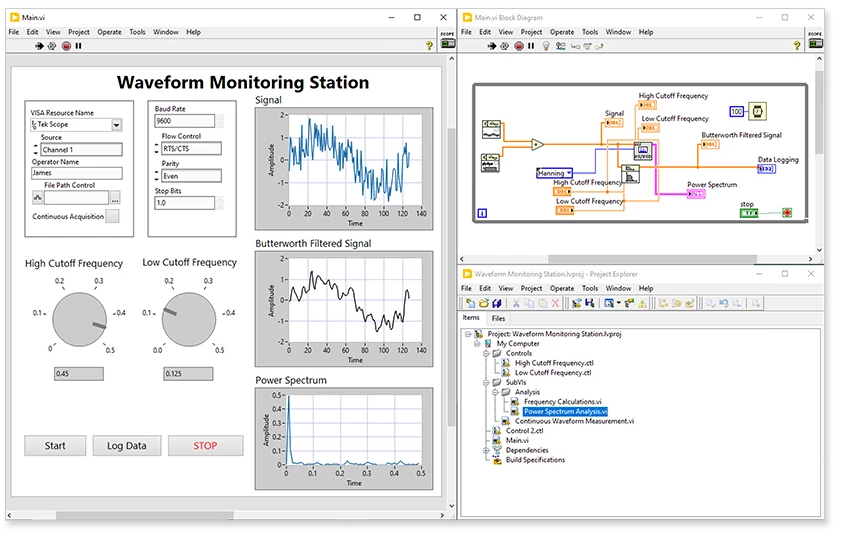
\includegraphics[width = 15cm]{images/labview.png}
 \caption{Przykładowy interfejs stworzony przy pomocy LabView.} 
 \label{fig:labview_grafika}
\end{figure}

Do niewątpliwych zalet takiego rozwiązania należy zaliczyć możliwość wykorzystania posiadanego już sprzętu, a także łatwość rozbudowy i przystosowania do innego typu pomiarów.
Niestety, może się okazać, że wykorzystywane instrumenty nie posiadają łatwo dostępnego API, które umożliwiałoby integrację. Nierzadko przeszkodę stanowi także samo środowisko, do którego użycia niejako zmusza producent.